\documentclass{article}
\usepackage{hyperref}
\usepackage{graphicx}
\usepackage[margin=1.5cm]{geometry}
\usepackage{amsmath}

\begin{document}
\twocolumn

\title{Warm Up Exercises: Unit 2, Forces II}
\author{Prof. Jordan C. Hanson}

\maketitle

\begin{figure}[ht]
\centering
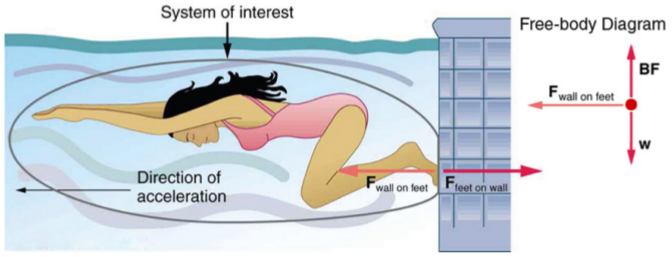
\includegraphics[width=0.45\textwidth]{figures/wall.png}
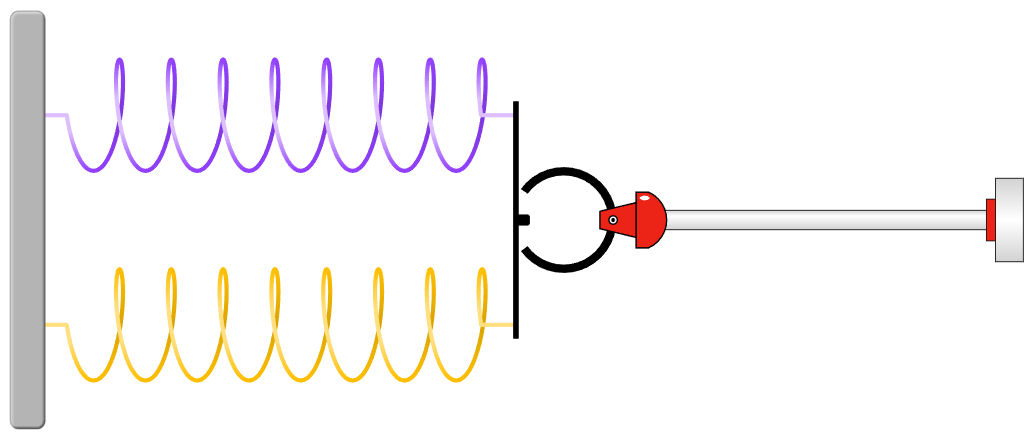
\includegraphics[width=0.45\textwidth]{figures/parallel_springs.png}
\caption{\label{fig:1} (Top) A swimmer pushes off the wall underwater. (Bottom) Two springs connected in parallel.}
\end{figure}

\section{Memory Bank}

\begin{enumerate}
\item $\vec{F} = m \vec{a}$ ... Newton's 2nd Law
\item $\vec{F}_{\rm AB} = -\vec{F}_{\rm BA}$ ... Newton's 3rd Law
\item $\vec{s} = -k \Delta \vec{x}$ ... Hooke's Law (spring force)
\item $\vec{f} = -\mu N \hat{i}$ ... Force of friction along horizontal
\item $\vec{F}_{\rm C} = - m \vec{r} \omega^2$ ... Centripetal force
\item $\vec{F}_{\rm C} = -(mv^2/r)\hat{r}$ ... Centripetal force
\end{enumerate}

\section{Chapter 5 - Forces I}

\begin{enumerate}
\item (a) What net external force is exerted on a 1100.0 kg artillery shell fired from a battleship if the shell is accelerated at $2.40\times 10^4$ m s$^{-2}$? (b) What is the magnitude of the force exerted on the ship by the artillery shell, and why? (c) What is the acceleration of the battleship, if its mass is $5\times 10^7$ kg? \\ \vspace{3cm}
\item A swimmer pushes backward on an underwater wall (Fig. \ref{fig:1}, top) with force of 800.0 N. The mass of the swimmer is 50 kg.  (a) What is the acceleration of the swimmer? (b) Why does the swimmer accelerate to the \textit{left}, if her applied force is to the \textit{right?} \\ \vspace{2cm}
\item (a) If a 180 kg rugby player hits a 120 kg player, what is the ratio of their accelerations? (b) If the acceleration of the heavier player is observed to be +0.5 m s$^{-2}$, what is the acceleration of the lighter player? \\ \vspace{1cm}
\end{enumerate}

\section{Chapter 6 - Forces II}

\begin{enumerate}
\item Three forces act on an object, considered to be a particle, which moves with constant velocity $\vec{v} = 3\hat{i} - 2\hat{j}$ m s$^{-1}$.  Two of the forces are $\vec{F}_1 = 3\hat{i} + 5\hat{j}$ N and $\vec{F}_2 = 4\hat{i} - 7\hat{j}$ N.  Find the third force. \\ \vspace{3cm}
\item Consider Fig. \ref{fig:1} (bottom).  The two springs are connected \textit{in parallel}.  (a) If the k-value of each spring is 100 N m$^{-1}$, what force would each provide if stretched by 10 cm?  (b) If connected in parallel, with what force would we have to pull to measure a displacement of 20 cm? (c) Consider the simulation to compare a single spring to two springs connected in parallel: \small \url{https://phet.colorado.edu/en/simulations/hookes-law} \normalsize
\end{enumerate}

\end{document}
